\documentclass[11pt]{article}

\usepackage{a4wide}
\usepackage[utf8]{inputenc}
\usepackage[russian]{babel}
\usepackage{graphicx}
\usepackage{amsmath}
\usepackage{amsthm}
\usepackage{amssymb}
\usepackage[section]{placeins}

\newtheorem{theorem}{Теорема}
\newtheorem{definition}{Определение}
\newtheorem{proposition}{Утверждение}

\newcommand*{\hm}[1]{#1\nobreak\discretionary{}{\hbox{$\mathsurround=0pt #1$}}{}}
\newcommand\abs[1]{\left\lvert#1\right\rvert}
\newcommand{\scalar}[2]{\left<#1,#2\right>}
\newcommand{\norm}[1]{\left\lVert #1 \right\lVert}
\newcommand{\const}{\ensuremath{\operatorname{const}}}
\newcommand{\sgn}{\ensuremath{\operatorname{sgn}}}
\renewcommand{\d}[1]{\ensuremath{\operatorname{d}\!{#1}}}

\begin{document}
\thispagestyle{empty}

\begin{center}
\ \vspace{-3cm} \newline

\includegraphics[width=0.5\textwidth]{msu.eps}\\
{\scshape Московский государственный университет имени М.~В.~Ломоносова}\\
Факультет вычислительной математики и кибернетики\\
Кафедра системного анализа

\vfill

{\LARGE Отчёт по практикуму <<Динамическое программирование>>} \newline
%\vspace{1cm}
{\Huge\bfseries }
\end{center}

\vspace{1cm}
\begin{flushright}
\large
\textit{Студент 415 группы}\\
В.~С.~Терёшин\\
%\vspace{5mm}
%\textit{Руководитель практикума}\\
%к.ф.-м.н., доцент П.~П.~Петров
\end{flushright}

\vfill
\begin{center}
Москва, 2014
\end{center}
\pagebreak
\tableofcontents
\pagebreak
\section{Постановка задачи}
Дана колебательная система:

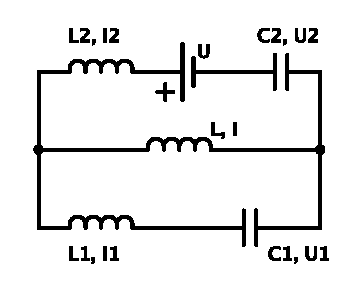
\includegraphics[scale=1.0]{circuit.eps}

Можно подавать напряжение $\abs{U} \leqslant \tilde{U}$. Известны начальные данные: $I_1^0, I_2^0, U_1^0, U_2^0$ и параметры элементов цепи: $L, L_1, L_2$.

Для данной системы необходимо вывести уравнения движения, описать характер движения системы без управления. Также с помощью \texttt{Matlab} и \texttt{Ellipsoidal Toolbox} необходимо создать иллюстрации к полученным формулам.
\section{Теоретические выкладки}
\subsection{Общие сведения из динамического программирования}
Рассмотрим задачу:
$$
\left\{
\begin{aligned}
\dot{x}(t) = A(t)x(t) + B(t)u(t), \\
x(t_0) \in \mathcal{E}(x_0, X_0), \\
u(t) \in \mathcal{E}(q(t), Q(t)), \\
u(t) \in \mathbb{R}^m, \; x(t) \in \mathbb{R}^n.
\end{aligned}\right.
$$

\begin{definition}[Эллипсоид]
Пусть $q \in \mathbb{R}^n$ и $Q \in \mathbb{R}^{n \times n}, Q = Q' \geqslant 0$. Тогда эллипсоидом $\mathcal{E}(q, Q)$ называется множество
$$
\mathcal{E}(q, Q) = \left\{ x \in \mathbb{R}^n \mid \scalar{l}{x} \leqslant \scalar{l}{q} + \scalar{l}{Ql}^{\tfrac{1}{2}} \right\}.
$$
\end{definition}

Из определения непосредственно следует выражение для опорной функции эллип-
соида:
$$
\rho(l \mid \mathcal{E}(q, Q)) = \scalar{l}{q} + \scalar{l}{Ql}^{\frac{1}{2}}.
$$

\begin{proposition}
$A\mathcal{E}(q, Q) = \mathcal{E}(Aq, AQA'), \; \forall A \in \mathbb{R}^{n \times n}$.
\end{proposition}

\begin{proposition}
Пусть $\mathcal{E}_1 = \mathcal{E}(q_1, Q_1)$ и $\mathcal{E}_2 = \mathcal{E}(q_2, Q_2)$ --- невырожденные эллипсоиды. Определим
$$
\mathcal{E}^+[l] = \mathcal{E}(q_1 + q_2, Q^+[l]), \; Q^+[l] = \left( \scalar{l}{Q_1 l}^{\frac{1}{2}} + \scalar{l}{Q_2 l}^{\frac{1}{2}} \right) \left( \frac{Q_1}{\scalar{l}{Q_1 l}^{\frac{1}{2}}} + \frac{Q_2}{\scalar{l}{Q_2 l}^{\frac{1}{2}}} \right).
$$
Тогда
\begin{enumerate}
\item $\forall l \rho(l \mid \mathcal{E}^+[l_0]) \geqslant \rho(l \mid \mathcal{E}_1 + \mathcal{E}_2)$;
\item $\rho(\pm l_0 \mid \mathcal{E}^+[l_0]) = \rho(\pm l_0 \mid \mathcal{E}_1 + \mathcal{E}_2)$.
\end{enumerate}
\end{proposition}
Из этого утверждения следует представление
$$
\mathcal{E}_1 + \mathcal{E}_2 = \bigcap\limits_{l \in \mathbb{S}_1(0)} \mathcal{E}^+(l),
$$
где $\mathbb{S}_1(0)$ --- единичная сфера с центром в $0$.

\begin{definition}
Множеством достижимости $\mathcal{X}[t] = \mathcal{X}(t; t_0, X_0, \mathcal{U})$ данной системы называется множество концов траекторий системы, отвечающих всем возможным допустимым
управлениям и всем возможным начальным данным:
$$
\mathcal{X}[t] = \bigcup\limits_{x_0 \in X_0} \bigcup\limits_{u(\cdot) \in \mathcal{U}} \left\{ x(t; t_0, x_0, u(\dot)) \right\}.
$$
\end{definition}

\begin{definition}
Трубкой достижимости системы называется многозначное отображение $T(t) = \left\{ (\tau, x) \in \mathbb{R}^{n+1} \mid \tau \in [t_0, t], x \in \mathcal{X}[\tau] \right\}$.
\end{definition}

Для рассматриваемой системы решения задаются формулой Коши:
$$
x(t) = X(t, t_0)x_0 + \int\limits_{t_0}^{t} X(t, \tau)B(\tau)u(\tau)d\tau.
$$
Откуда можно получить представление для множества достижимости системы:
\begin{gather}
\mathcal{X}[t] = X(t, t_0)\mathcal{E}(x_0, X_0) + \int\limits_{t_0}^t X(t, \tau)B(\tau)\mathcal{E}(q(\tau), Q(\tau))d\tau = \notag \\
= \mathcal{E}(g_0(t), G_0(t)) + \int\limits_{t_0}^t \mathcal{E}(g(t, \tau), G(t, \tau))d\tau, \notag
\end{gather}
где
\begin{gather}
g_0(t) = X(t, t_0)x_0, \notag \\
G_0(t) = X(t, t_0) X_0 X'(t, t_0), \notag \\
g(t, \tau) = X(t, \tau) B(\tau) q(\tau), \notag \\
G(t, \tau) = X(t, \tau) B(\tau) Q(\tau) B'(\tau) X'(t, \tau). \notag
\end{gather}
\subsection{Вывод уравнения движения системы}
Выписывая правила Кирхгофа для данной системы, получим:
\begin{gather}
U_2 + L\frac{dI}{dt} + L_2\frac{dI_2}{dt} = U, \notag \\
L\frac{dI}{dt} - L_1\frac{dI_1}{dt} = U_1, \notag
\end{gather}
Заметим, что $I=I_2-I_1$, и получим:
\begin{gather}
U_2 + L\frac{dI_2}{dt} - L\frac{dI_1}{dt} + L_2\frac{dI_2}{dt} = U, \notag \\
L\frac{dI_2}{dt} -L\frac{dI_1}{dt} - L_1\frac{dI_1}{dt} = U_1, \notag
\end{gather}

Получили систему линейных дифференциальных уравнений относительно $\frac{dI_1}{dt}$ и  $\frac{dI_2}{dt}$. Её можно разрешить относительно $\frac{dI_1}{dt}$ и  $\frac{dI_2}{dt}$:
\begin{gather}
D = L_1 L_2 + L(L_1 + L_2), \notag \\
\frac{dI_1}{dt} = -\frac{L+L2}{D}U_1 - \frac{L}{D}U_2 + \frac{L}{D}U, \notag \\
\frac{dI_2}{dt} = -\frac{L}{D}U_1 - \frac{L+L1}{D}U_2 + \frac{L+L1}{D}. \notag
\end{gather}

Добавим равенство сил тока на последовательном соединении конденсатора $C_1$ и катушки $L_1$, а также на последовательном соединении конденсатора $C_2$ и катушки $L_2$:
\begin{gather}
\left\{
\begin{aligned}
\frac{dI_1}{dt} = -\frac{L+L_2}{D}U_1 - \frac{L}{D}U_2 + \frac{L}{D}U, \notag \\
\frac{dI_2}{dt} = -\frac{L}{D}U_1 - \frac{L+L_1}{D}U_2 + \frac{L+L_1}{D}, \notag \\
\frac{dU_1}{dt} = \frac{I_1}{C_1}, \notag \\
\frac{dU_2}{dt} = \frac{I_2}{C_2}. \notag
\end{aligned}
\right.
\end{gather}

Введём обозначения: $x_1 = I_1, x_2 = I_2, x_3 = U_1, x_4 = U_2$:
\begin{gather}
\left\{
\begin{aligned}
\dot{x_1} = -\frac{L+L_2}{D}x_3 - \frac{L}{D}x_4 + \frac{L}{D}U, \notag \\
\dot{x_2} = -\frac{L}{D}x_3 - \frac{L+L_1}{D}x_4 + \frac{L+L_1}{D}, \notag \\
\dot{x_3} = \frac{x_1}{C_1}, \notag \\
\dot{x_4} = \frac{x_2}{C_2}. \notag
\end{aligned}
\right.
\end{gather}

Эту систему можно записать в виде:
$$
\dot{x} = \begin{bmatrix}
0 & 0 & -\frac{L+L_2}{D} & -\frac{L}{D} \\
0 & 0 & -\frac{L}{D} & -\frac{L+L1}{D} \\
\frac{1}{C_1} & 0 & 0 & 0 \\
0 & \frac{1}{C_2} & 0 & 0
\end{bmatrix} x + 
\begin{bmatrix}
\frac{L}{D} \\
\frac{L+L1}{D} \\
0 \\
0
\end{bmatrix} u
$$
и начальных данных:
$$
x_0 = \begin{bmatrix}
I_1^0 \\
I_2^0 \\
U_1^0 \\
U_2^0 \\
\end{bmatrix}.
$$
\subsection{Использование \texttt{Ellipsoidal Toolbox}}
Для численного решения данной задачи воспользуемся \texttt{Ellipsoidal Toolbox} для среды программирования \texttt{Matlab}.

Данный набор инструментов позволяет строить внутренние и внешние эллипсоидальные оценки множеств, обеспечивает необходимыми функциями для работы с эллипсоидальным исчислением и обладает средствами вывода полученных результатов в виде графикоф.

Одной из важных функций \texttt{Ellipsoidal Toolbox} является \texttt{elltool.reach.ReachContinuous}, позволяющая решать данную задачу. Для корректной работы данной функции необходимо указать систему, начальные данные, временной интервал, шаг разбиения временного интервала, направления для расчётов внешних или внутренних эллипсоидальных оценок, а также требуемые абсолютные и относительные погрешности (\texttt{elltool.reach.ReachContinuous} использует в своей работе функцию \texttt{ode45}).
\subsection{Погрешности}
При работе над данной задачи средствами \texttt{Ellipsoidal Toolbox} возникают следующие погрешности:
\begin{enumerate}
\item Погрешность из-за дискретизации времени возникает из-за принципиальной невозможности решения непрерывных задач средствами современных компьютеров. При решении задачи средствами \texttt{Ellipsoidal Toolbox} происходило разбиение времени на 1000 частей.
\item Погрешность ограниченного количества направлений для построения внешних или внутренних эллипсоидальных оценок.
\item Погрешности операций над числами с плавающей точкой.
\end{enumerate}

В следующем параграфе будут приведены абсолютные и относительные погрешности для приведённого примераю.
\section{Примеры работы программы}
\subsection{Поведение системы без управления}
Рассматриваются начальные данные: $L = 1.0, L_1 = 2.0, L_2 = 3.0, C_1 = 2.0, C_2 = 2.5, I_1^0 = 1.0, I_2^0 = 1.0, U_1^0 = 1.0, U^2_0 = 1.0, \tilde{U} = 5.0$.

\includegraphics[scale=0.8]{pics/no_control_x1.eps}

\includegraphics[scale=0.8]{pics/no_control_x2.eps}

\includegraphics[scale=0.8]{pics/no_control_x3.eps}

\includegraphics[scale=0.8]{pics/no_control_x4.eps}

Данное поведение системы можно объяснить тем, что электрические цепи из катушек индуктивности и конденсаторов без сопротивления подвержены колебаниям.
\subsection{Поведение системы при наличии управления}
\subsubsection{Пример 1}
Рассматриваются начальные данные: $L = 1.0, L_1 = 2.0, L_2 = 3.0, C_1 = 3.0, C_2 = 2.5, I_1^0 = 0.1, I_2^0 = 0.5, U_1^0 = 0.5, U^2_0 = 0.3, \tilde{U} = 2.0$. Используется 40 внешних оценок.

\includegraphics[scale=0.7]{pics/control_1.eps}
\includegraphics[scale=0.7]{pics/control_projection_1.eps}

Полученный результат: минимальное время, требующееся для успокоения системы, примерно равно $20.3030$. Абсолютная погрешности равна $10^{-7}$, относительная $10^{-5}$.
\subsubsection{Пример 2}
Рассматриваются начальные данные: $L = 5.0, L_1 = 1.0, L_2 = 3.0, C_1 = 1.0, C_2 = 4.0, I_1^0 = 0.2, I_2^0 = 0.2, U_1^0 = 0.1, U^2_0 = 0.1, \tilde{U} = 1.0$. Используется 40 внешних оценок.

\includegraphics[scale=0.7]{pics/control_2.eps}
\includegraphics[scale=0.7]{pics/control_projection_2.eps}

Полученный результат: минимальное время, требующееся для успокоения системы, примерно равно $4.2424$. Абсолютная погрешности равна $10^{-7}$, относительная $10^{-5}$.
\pagebreak
\addcontentsline{toc}{section}{Список литературы}
\begin{thebibliography}{99}
	\bibitem{EllToolMan} П.~Гагаринов, А.~А.~Куржанский: Инструкция к Ellipsoidal Toolbox, 2014.
\end{thebibliography}
\end{document}
